\documentclass[%margin%,line,pifont,palatino,courier
]{article}
\usepackage{fullpage}
\usepackage{lastpage}
\usepackage[top=1in,bottom=1in,margin=1in]{geometry}
\usepackage{supertabular}
\usepackage{graphicx,tikz}	
%\usepackage{tkz-euclide}
%\usetkzobj{all}
%\usetikzlibrary{calc}
\usepackage{array,multicol}
\usepackage{amsmath,amssymb}
\usepackage{enumitem}
\usepackage{framed}

\usepackage{fancyhdr}
\pagestyle{fancy}

\addtolength{\topmargin}{-0.25in}

\newcommand{\vect}[1]{\mathbf{#1}}
\DeclareMathOperator{\proj}{proj}

\fancypagestyle{plain}{
	\addtolength{\headheight}{0.485in}
	\rhead{\bf MATH 2574 (Calculus III) \\
		%\vspace{0.5pc}
		due Mon 27 Feb 2017 \\}
	\rfoot{\footnotesize $\;$Quiz 3TH, p. \thepage\ (of \pageref{LastPage})
	}
\renewcommand{\headrulewidth}{0pt}
}
\fancyhf{}
\renewcommand{\headrulewidth}{0pt}
\rfoot{\footnotesize Quiz 3TH, p. \thepage\ (of \pageref{LastPage})$\;$}

\title{\vspace{-3.5pc} 
	\flushleft \bf \Large Take-Home Quiz 3: \\ Derivatives in multivariables (\S 12.4-12.8)}
\date{}

% % % % %
\begin{document}
\maketitle

\vspace{-3pc}
\noindent{\bf Directions:} This quiz is due on February 27, 2017 at the beginning of lecture.  You may use whatever resources you like -- e.g., other textbooks, websites, collaboration with classmates -- to complete it \textbf{but YOU MUST DOCUMENT YOUR SOURCES}.  Acceptable documentation is enough information for me to find the source myself.  Rote copying another's work is unacceptable, regardless of whether you document it.  

\noindent\hrulefill

\begin{enumerate}
% % %
\item {\bf 12.4 \#78} 
Traveling waves (for example, water waves or electromagnetic waves) exhibit periodic motion in both time and position.  In one dimension, some types of wave motion are governed by the one-dimensional wave equation
\[
\frac{\partial^2u}{\partial t^2}=c^2\frac{\partial^2u}{\partial x^2}
\]
where $u(x,t)$ is the height or displacement of the wave surface at position $x$ and time $t$, and $c$ is the constant speed of the wave. 

Show that $u(x,t)=5\cos(2(x+ct))+3\sin(x-ct)$ satisfies the wave equation.

\vspace{1pc}
% % %
\item {\bf 12.4 \#88}
The formal definition of differentiability is given as follows (p. 902):

%\hline
\begin{quote}
%\begin{framed}
\hrulefill

The function $z=f(x,y)$ is \textbf{differentiable at $(a,b)$} means $f_x(a,b)$ and $f_y(a,b)$ exist and the change $\Delta z=f(a+\Delta x,b+\Delta y)-f(a,b)$ equals
\[
f_x(a,b)\Delta x+f_y(a,b)\Delta y+\varepsilon_1\Delta x+\varepsilon_2\Delta y,
\]
where 
\begin{align*}
\varepsilon_1 &= \frac{f(a+\Delta x,b)-f(a,b)}{\Delta x}-f_x(a,b)\; \longrightarrow 0\qquad\text{as}\qquad \Delta x\to 0 \quad\text{and}\\
\varepsilon_2 &= \frac{f(a,b+\Delta y)-f(a,b)}{\Delta y}-f_y(a,b)\; \longrightarrow 0\qquad\text{as}\qquad \Delta y\to 0.
\end{align*}
%\end{framed}
\hrulefill
\end{quote}
%\hline 

For the function $z=f(x,y)=2x+3y^2$, let $(a,b)=(0,0)$.  Find:
\begin{enumerate}
	\item $\Delta z$ \textit{(Hint: Your answer should be in terms of $\Delta x$ and $\Delta y$.)}
	\item $f_x(a,b)$ and $f_y(a,b)$
	\item $\varepsilon_1$ and $\varepsilon_2$
\end{enumerate}

According to the definition of differentiable given above, is the function $z=f(x,y)=2x+3y^2$ differentiable at $(0,0)$?

%\item {\bf 12.5 \#18}
%The volume of a pyramid with a square base $x$ units on a side and a heigh of $h$ is $V=\frac{1}{3}x^2h$.
%\begin{enumerate}
%	\item Assume that $x=x(t)$ and $h=h(t)$ are functions of $t$ (time).  Find $V'(t)$.
%	\item Suppose that for $t\geq 0$,
%	\begin{align*}
%	x(t) &= \frac{t}{t+1} \quad\text{and} \\
%	h(t) &= \frac{1}{t+1}.
%	\end{align*}
%	Use your answer to part (a) to find $V'(t)$.
%	\item Does the volume of the pyramid in part (b) increase or decrease at $t$ increases?
%\end{enumerate}

\vspace{1pc}
% % %
\item {\bf 12.5 \#30}
Use a tree diagram (explained on p. 908) to write the required Chain Rule formula for $\dfrac{\partial u}{\partial z}$, given that
\[\begin{array}{c}
	u = f(v,w,x) \\
	v = g(r,s,t),\quad w = h(r,s,t),\quad x = p(r,s,t) \\
	r = F(z).
\end{array}\]

%\vspace{1pc}
% % %
\item {\bf 12.5 \#64}
Cartesian coordinates $(x,y)$ and \textbf{polar coordinates $(r,\theta)$} are related through the following transformation equations
\[
x = r\cos{\theta} \qquad y = r\sin{\theta}
\]
and 
\[
r^2 = x^2+y^2 \qquad \tan{\theta} = \frac{y}{x}.
\]
\begin{enumerate}
	\item Evaluate the partial derivatives $x_r,\,y_r,\,x_{\theta},\,y_{\theta}$.
	\item Evaluate the partial derivatives $r_x,\,r_y,\,\theta_x,\,\theta_y$ (assume $r\geq 0$).
	\item For a function $z=f(x,y)$, write the expressions for $z_r$ and $z_{\theta}$.%, where $x$ and $y$ are expressed in terms of $r$ and $\theta$.
	\item For a function $w=g(r,\theta)$, write the expressions for $w_x$ and $w_y$.%, where $r$ and $\theta$ are expressed in terms of $x$ and $y$.
\end{enumerate}

%\item {\bf 12.6 \#8}
%Consider the function $f(x,y)=2x^2+y^2$, whose graph is the following paraboloid:
%{\bf FIGURE}
%\begin{enumerate}
%	\item Fill in the table with the values of the directional derivative at the points $(a,b)$ in the directions given by the unit vectors $\vect u$, $\vect v$, and $\vect w$.
%	\[\begin{array}{l|l|l|l}
%	 & (a,b)=(1,0) & (a,b)=(1,1) & (a,b)=(1,2) \\
%	 \hline
%	 \vect u=\langle 1,0\rangle & & & \\
%	 \hline
%	 \vect v=\langle \frac{\sqrt{2}}{2}, \frac{\sqrt{2}}{2}\rangle & & & \\
%	 \hline
%	 \vect w=\langle 0,1\rangle & & &
%	\end{array}\]
%	\item Interpret each of the directional derivatives computed in part (a) at the point $(1,0)$.
%\end{enumerate}

\vspace{1pc}
% % %
\item {\bf 12.6 \#40}
Consider the function $f(x,y)=-4+6x^2+3y^2$ and the point $P=(-1,-2)$ in $\mathbb R^2$.  Sketch the $xy$-plane showing $P$ and the level curve of $f$ through $P$.  Then indicate the directions of maximum increase, maximum decrease, and no change for $f$.

\vspace{1pc}
% % %
\item {\bf 12.6 \#74}
The surface 
\[
f(x,y,z)=xy+xz-yz-1
\]
is a level surface of the function $w=f(x,y,z)$ (for $w=0$).
\begin{enumerate}
	\item Find the gradient of $f$ and evaluate it at the point $P=(1,1,1)$.
	\item The set of all vectors orthogonal to the gradient with their tails at $P$ forms the \textbf{tangent plane} of $f$ to $P$.  Find an equation of that plane.
\end{enumerate}

\vspace{1pc}
% % %
\item {\bf 12.7 \#60}
In general, real numbers (which usually have infinite decimal expansions) cannot be represented exactly in a computer by floating-point numbers (which have finite decimal expansions).  \textit{(In fact, that was the point of the Taylor estimations from Cal II!)}

Suppose that floating-point numbers on a particular computer carry an error of at most $10^{-16}$.  Estimate the maximum error that is committed in doing the following arithmetic operations.  Express the error in absolute ($dz$ for $z=f(x,y)$ or $dw$ for $w=F(x,y,z)$) and relative $\left(\left|\dfrac{\Delta z-dz}{\Delta z}\right|\text{ or }\left|\dfrac{\Delta w-dw}{\Delta w}\right|\right)$ terms.
\begin{enumerate}
	\item $f(x,y)=xy$
	\item $f(x,y)=\frac{x}{y}$
	\item $F(x,y,z)=xyz$
	\item $F(x,y,z)=\dfrac{\frac{x}{y}}{z}$
\end{enumerate}

%\item {\bf 12.7 \#62}
%When two electrical resistors with resistance $R_1>0$ and $R_2>0$ are wired in parallel in a circuit (see figure), the combined resistance $R$, measured in ohms ($\Omega$), is given by
%\[
%\frac{1}{R}=\frac{1}{R_1}+\frac{1}{R_2}.
%\]
%\begin{enumerate}
%	\item Estimate the change in $R$ if $R_1$ increases from $2\,\Omega$ to $2.05\,\Omega$ and $R_2$ decreases from $3\,\Omega$ to $2.95\,\Omega$.
%	\item Is it true that if $R_1=R_2$ and $R_1$ increases by the same small amount that $R_2$ decreases, then $R$ is approximately unchanged?  Explain.
%	\item Is it true that if $R_1$ and $R_2$ increase, then $R$ increases?  Explain.
%	\item Suppose $R_1>R_2$ and $R_1$ increases by the same small amount the $R_2$ decreases.  Does $R$ increase or decrease?
%\end{enumerate}

\vspace{1pc}
% % %
\item {\bf 12.8 \#70}
%In its many guises, the \textbf{least squares appoximation} arises in numerous areas of mathematics and statistics.  
Suppose you collect data for two variables $x$ and $y$ (e.g., height and shoe size) in the form of pairs $(x_1,y_1),(x_2,y_2),\dots,(x_n,y_n)$ (so there are $n$ data points).  This data may be plotted as a scatterplot in the $xy$-plane, as shown in the figure:

\begin{center}
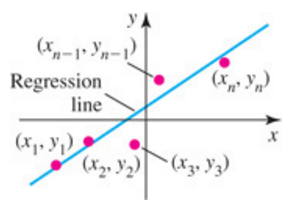
\includegraphics{Q3regression}
\end{center}

The technique known as \textbf{linear regression} asks the question: What is the equation of the line that ``best fits" the data (the blue line in the figure)?  The \textbf{least squares criterion} for best fit requires that the sum of the squares of the vertical distances between the line and the data points is a minimum.  The equation of the best fit (or \textbf{regression}) line has the form $y=mx+b$, where the slope $m$ and the $y$-intercept $b$ are determined by the least squares condition.

Suppose you are given the three data points $(x_1,y_1)=(1,2)$, $(x_2,y_2)=(3,4)$, and $(x_3,y_3)=(5,6)$.
\begin{enumerate}
	\item The sum of the squares of the vertical distances between the regression line and the data points is a function of $m$ and $b$:
	\[
	F(m,b)=((m+b)-2)^2+(3m+b)-5)^2+((4m+b)-6)^2
	\]
	Briefly explain where this formula comes from.
	\item Find the critical points of $F$ and the values of $m$ and $b$ that minimize $F$.
	\item Graph the three data points and the regression line.
\end{enumerate}



% % % % %
\end{enumerate}
\end{document}